%% !TeX program = xelatex
% svg를 써야 해서 부득이하게 pdflatex 사용

%%%%%%%%%%%%%%%%%%%%%%%%%%%%%%%%%%%%%%%%%%%%%%%%%%%%%%%%%%%%%%%%%%%%%%%%%
%%%  LaTeX format of the thesis of the Gyeonggi Science High School   %%%
%%%  Last edition 2015.11.13 by Chinook Mok                           %%%
%%%  Continously being modified by gshslatexintro after 2016.02.02.   %%%
%%%  Check webpage http://gshslatexintro.github.io                    %%%
%%%  Also refer to https://www.facebook.com/gshstexsociety            %%%
%%%%%%%%%%%%%%%%%%%%%%%%%%%%%%%%%%%%%%%%%%%%%%%%%%%%%%%%%%%%%%%%%%%%%%%%%

\documentclass[twoside,11pt]{gshs_thesis}
\usepackage{subcaption}
\usepackage[per-mode=symbol]{siunitx}
\sisetup{inter-unit-product =$\cdot$} % http://tex.stackexchange.com/questions/59032/how-to-format-si-units
%\usepackage[hidelinks]{hyperref}
\usepackage{verbatim}
\usepackage{indentfirst}
\usepackage{diagbox}
\captionsetup{subrefformat=parens}
\graphicspath{{../images/}}
%\captionsetup[figure]{font=small,skip=10pt}
\renewcommand\figurename{Fig.}
\usepackage{enumitem}
\setitemize{noitemsep} % for reducing line space in itemize environments
\setenumerate{noitemsep} % for reducing line space in enumerate environments
%\usepackage[hidelinks]{hyperref}
%\hypersetup{pdfencoding=auto,bookmarks}
%\usepackage{bookmark}
%\usepackage{tocloft}
%\cftpagenumbersoff{section}
%\setcounter{secnumdepth}{2} % toc에는 subsubsection을 제외
%\setcounter{tocdepth}{2}
\usepackage{array}
%\usepackage{multirow}
\newcommand{\nocontentsline}[3]{}
\newcommand{\tocless}[2]{\bgroup\let\addcontentsline=\nocontentsline#1{#2}\egroup}

\newcommand{\etal}{{\it et al.}}
\newcommand{\etalspace}{{\it et al. }}
\newcommand{\scp}{SCP artificial muscle }
\newcommand{\SCP}{SCP Artificial Muscle }
\newcommand{\ANTA}{Antagonistic Robot Arm }
\newcommand{\Anta}{Antagonistic robot arm } 
\newcommand{\anta}{antagonistic robot arm }
\newcommand{\APC}{Antagonistic Position Control }
\newcommand{\Apc}{Antagonistic position control }
\newcommand{\apc}{antagonistic position control }
\newcommand{\scpnospace}{SCP artificial muscle} 
\newcommand{\SCPnospace}{SCP Artificial Muscle}
\newcommand{\ANTAnospace}{Antagonistic Robot Arm}
\newcommand{\Antanospace}{Antagonistic robot arm} 
\newcommand{\antanospace}{antagonistic robot arm}
\newcommand{\APCnospace}{Antagonistic Position Control}
\newcommand{\Apcnospace}{Antagonistic position control}
\newcommand{\apcnospace}{antagonistic position control}
\newcommand{\needcitation}{[Citation Needed]}
\newcommand{\scps}{SCP artificial muscles }
\newcommand{\scpsnospace}{SCP artificial muscles}
\newcommand{\ANTAs}{Antagonistic Robot Arms } 
\newcommand{\antas}{antagonistic robot arms }
\newcommand{\antasnospace}{antagonistic robot arms}
\newcommand{\Antas}{Antagonistic robot arms }
\newcommand{\Antasnospace}{Antagonistic robot arms}

% -----------------------------------------------------------------------
%                   이 부분은 수정하지 마시오.
% -----------------------------------------------------------------------
\titleheader{졸업논문청구논문}
\school{과학영재학교 경기과학고등학교}
\approval{위 논문은 과학영재학교 경기과학고등학교 졸업논문으로\\
졸업논문심사위원회에서 심사 통과하였음.}
\chairperson{심사위원장}
\examiner{심사위원}
\apprvsign{(인)}
\korabstract{초 록}
\koracknowledgement{감사의 글}
\korresearches{연 구 활 동}

%: ----------------------------------------------------------------------
%:                  논문 제목과 저자 이름을 입력하시오
% ----------------------------------------------------------------------
\title{SCP로 작동하는 Antagonistic Robot Arm의 공냉에 의한 지속 가능한 제어} %한글 제목
\engtitle{SCP-Powered Antagonistic Robot Arm's Sustainable Control by Forced Air-Cooling} %영문 제목
\korname{박 승 원} %저자 이름을 한글로 입력하시오 (글자 사이 띄어쓰기)
\engname{Park, Seung-Won} %저자 이름을 영어로 입력하시오 (family name, personal name)
\chnname{朴 承 元} %저자 이름을 한자로 입력하시오 (글자 사이 띄어쓰기)
\studid{14041} %학번을 입력하시오

%------------------------------------------------------------------------
%                  심사위원과 논문 승인 날짜를 입력하시오
%------------------------------------------------------------------------
\advisor{Oh, Jeonghyeon}  %지도교사 영문 이름 (family name, personal name)
\judgeone{문 형 필} %심사위원장
\judgetwo{남 태 정}   %심사위원1
\judgethree{오 정 현} %심사위원2(지도교사)
\degreeyear{2017}   %졸업 년도
\degreedate{2016}{X}{X} %논문 승인 날짜 양식1
%\degreedatekor{2016년 X월 X일} %논문 승인 날짜 양식2

%------------------------------------------------------------------------
%                  논문제출 전 체크리스트를 확인하시오
%------------------------------------------------------------------------
\checklisttitle{[논문제출 전 체크리스트]} %수정하지 마시오
\checklistI{1. 이 논문은 내가 직접 연구하고 작성한 것이다.} %수정하지 마시오
% 이 항목이 사실이라면 다음 줄 앞에 "%"기호 삽입, 다다음 줄 앞의 "%"기호 제거하시오
%\checklistmarkI{$\square$}
\checklistmarkI{$\text{\rlap{$\checkmark$}}\square$}
\checklistII{2. 인용한 모든 자료(책, 논문, 인터넷자료 등)의 인용표시를 바르게 하였다.} %수정하지 마시오
% 이 항목이 사실이라면 다음 줄 앞에 "%"기호 삽입, 다다음 줄 앞의 "%"기호 제거하시오
%\checklistmarkII{$\square$}
\checklistmarkII{$\text{\rlap{$\checkmark$}}\square$}
\checklistIII{3. 인용한 자료의 표현이나 내용을 왜곡하지 않았다.} %수정하지마시오
% 이 항목이 사실이라면 다음 줄 앞에 "%"기호 삽입, 다다음 줄 앞의 "%"기호 제거하시오
%\checklistmarkIII{$\square$}
\checklistmarkIII{$\text{\rlap{$\checkmark$}}\square$}
\checklistIV{4. 정확한 출처제시 없이 다른 사람의 글이나 아이디어를 가져오지 않았다.} %수정하지 마시오
% 이 항목이 사실이라면 다음 줄 앞에 "%"기호 삽입, 다다음 줄 앞의 "%"기호 제거하시오
%\checklistmarkIV{$\square$}
\checklistmarkIV{$\text{\rlap{$\checkmark$}}\square$}
\checklistV{5. 논문 작성 중 도표나 데이터를 조작(위조 혹은 변조)하지 않았다.} %수정하지 마시오
% 이 항목이 사실이라면 다음 줄 앞에 "%"기호 삽입, 다다음 줄 앞의 "%"기호 제거하시오
%\checklistmarkV{$\square$}
\checklistmarkV{$\text{\rlap{$\checkmark$}}\square$}
\checklistVI{6. 다른 친구와 같은 내용의 논문을 제출하지 않았다.} %수정하지 마시오
% 이 항목이 사실이라면 다음 줄 앞에 "%"기호 삽입, 다다음 줄 앞의 "%"기호 제거하시오
%\checklistmarkVI{$\square$}
\checklistmarkVI{$\text{\rlap{$\checkmark$}}\square$}

 % usepackage 등의 명령어는 여기에.


\usepackage{tocloft}
\setlength{\cftbeforesecskip}{0pt}
\setlength{\cftbeforesubsecskip}{0pt}
\setlength{\cftbeforesubsubsecskip}{0pt}

\begin{document}
	%	\renewcommand\baselinestretch{1.2} % line spacing in the paragraph
	\baselineskip=2.2em         % line spacing in the paragraph
	
	%\renewcommand\baselinestretch{1.2} % line spacing in the paragraph
%\baselineskip=22pt plus1pt         % line spacing in the paragraph

\maketitle  % command to print the title page with above variables
\setcounter{page}{1}
%---------------------------------------------------------------------
%                  영문 초록을 입력하시오
%---------------------------------------------------------------------
\begin{abstracts}     %this creates the heading for the abstract page
\noindent{
Recently discovered Super-Coiled Polymer(SCP) artificial muscle is being widely studied for next generation actuator due to its striking performance and low cost. There had been established general method for heating \scpnospace, but not yet for cooling in efficient and precise way. In this paper, \scpnospace's character is analysed and confirmed, and \anta - which is suitable for various tasks - were made and its position was controlled to make desired movement with 6.7\% error. Also, compressed air can and solenoid valve are controlled to feedback control the thermal conductivity. Finally, two-period \apc was demonstrated, and feedback cooling was simulated, confirming that \apc can be sustainable.
}
\end{abstracts}

%---------------------------------------------------------------------
%                  국문 초록을 입력하시오
%---------------------------------------------------------------------
\begin{abstractskor}        %this creates the heading for the abstract page
\noindent{
최근 발견된 super-coiled polymer(SCP) artificial muscle은 기존의 인공근육에 비해 월등한 성능과 낮은 단가를 가져 미래 로봇 산업을 이끌어갈 재료로 주목을 받고 있다. 온도에 반응하는 \scpnospace 을 가열하기 위한 방법은 정립되었으나, 냉각을 위한 효율적이고 정확한 방법은 세워지지 않았다. 본 논문에서는 \scpnospace 의 특성을 모델링하고 검증하였으며, 다양한 상황에 대응 가능한 \anta 를 제작하여 원하는 각도를 따라 6.7\%의 오차로 구동하였다. 또한, 압축공기와 솔레노이드 밸브의 개폐를 조절하여 열전도도를 feedback 제어할 수 있도록 하였다. 최종적으로는 두 주기 \apcnospace 을 시연하고, feedback 냉각을 전산모사하여 \apcnospace 이 지속 가능함을 확인하였다.
}
\end{abstractskor}


%----------------------------------------------
%   Table of Contents (자동 작성됨)
%----------------------------------------------
\setcounter{secnumdepth}{3} % organisational level that receives a numbers
\setcounter{tocdepth}{3}    % print table of contents for level 3
\tableofcontents


%----------------------------------------------
%     List of Figures/Tables (자동 작성됨)
%----------------------------------------------
\cleardoublepage
\clearpage
\listoffigures	% 그림 목록과 캡션을 출력한다. 만약 논문에 그림이 없다면 이 줄의 맨 앞에 %기호를 넣어서 코멘트 처리한다.

\cleardoublepage
\clearpage
\listoftables  % 표 목록과 캡션을 출력한다. 만약 논문에 표가 없다면 이 줄의 맨 앞에 %기호를 넣어서 코멘트 처리한다.


%%%%%%%%%%%%%%%%%%%%%%%%%%%%%%%%%%%%%%%%%%%%%%%%%%%%%%%%%%%
%%%% Main Document %%%%%%%%%%%%%%%%%%%%%%%%%%%%%%%%%%%%%%%%
%%%%%%%%%%%%%%%%%%%%%%%%%%%%%%%%%%%%%%%%%%%%%%%%%%%%%%%%%%%
\cleardoublepage
\clearpage
\renewcommand{\thepage}{\arabic{page}}
\setcounter{page}{1} % Abstract
	
	%%%%%%%%%%%%%%%%%%%%%%%%%%%%%%%%%%%%%%%%%%%%%%%%%%%%%%%%%%%
	%%%% Main Document %%%%%%%%%%%%%%%%%%%%%%%%%%%%%%%%%%%%%%%%
	%%%%%%%%%%%%%%%%%%%%%%%%%%%%%%%%%%%%%%%%%%%%%%%%%%%%%%%%%%%
	
	%-----------------------------------------------------
%  Introduction
%-----------------------------------------------------

\section{Introduction}
Artificial muscles have been vastly studied in Robotics to perform human's delicate movements \cite{ashley}. Recently, a super-coiled polymer(SCP) artificial muscle and its striking features were discovered by Haines \etal \cite{haines} The \scp is a new kind of artificial muscles which can be easily fabricated by simply twisting a nylon thread excessively. This artificial muscle contracts when heated while it relaxes when cooled.

It is known \scps can provide fast, nonhysteretic, strong, and large stroke at low costs\cite{yuan, mirvakili, madden}. 
Since the \scp was announced in 2014, it has been widely studied in many different fields, such as its application on
wearable robots \cite{sphincter, kianzad2}, 
anthropomorphic robotic hands \cite{yip, finger}, 
and modeling of its mechanism \cite{treatise, torsional, youngmodulus, fab_coil, multiscale, healing, kianzad, moretti}. 
%However, appropriate circumstances for SCP artificial muscle%, especially cooling device, 
%hadn't been studied enough to apply this artificial muscle into real robots.
However, the \scps have failed to be examined in appropriate circumstances enough to apply these artificial muscles into real robots.

Haines \etalspace present \scpnospace's heating method - fabricating the \scps with silver coated nylon thread and applying electric current, which provides Joule heat to muscles \cite{haines}. This method was checked and applied by several works \cite{yip, mirvakili,kianzad,sphincter,kianzad2}. However, methods for cooling \scps have been largely unsuccessful to date. 
Although water flow has been tried many times \cite{haines,finger},
it causes \scps not to last for a long time \cite{haines}.
%and it is hard to be applied to robots. 
%Furthermore, the application of the process to robots is rather difficult.
%Also, cooling fan was used in Yip \etal, but it didn't get sufficiently fast cooling speed.
Yip \etalspace also used a cooling fan in their study \cite{yip}, but it couldn't obtain sufficiently fast cooling speed.
% Thermo Neslab cc65 immersion cooler in \cite{kianzad}
% Liquid Nitrogen in Ionov.
% 'Electrical heating combined with compressed air or water for cooling are natural choices in the operating room. : Madden2015 : `Twisted Lines
Furthermore, there has been no study about feedback control of cooling speed.

In this paper, \antanospace, which is actuated by two complementarily contracting \scpsnospace, was assembled and its operating system was attached. Also, behaviors of the \scps and \anta were simply modeled with linear equations and tested experimentally. By quantifying thermal conductivity, possibility of feedback cooling was confirmed. In conclusion, algorithms for the sustainable \apc were designed, performed, and simulated. % Introduction
	
	\section{Preparation for the Muscles and the System}\label{section_preparation}
\scps respond to a function of temperature. In order to precisely control the complicated system, an electrical microprocessor was used. Therefore, the method for electrically operating \scps and investigating their characteristics is discussed in this section. 

\subsection{Fabrication of the SCP Artificial Muscles}
The \scps used in this paper were made by twisting silver-painted nylon thread (Conductive Sewing Thread Size 92, Shieldex), which was found to be best in terms of strain and force production \cite{haines}. First, the conductive thread was piled up four times to make its length be \SI{50}{\centi\meter}. Each side of thread was connected to washers. Then, a wire was hung to one of the washer and a motor to the other. (Fig.\ref{silverSCP_2})
As illustrated in Fig.\ref{silverSCP_illust}, the motor was rotated until the thread creates a coil \cite{fab_coil}. After making same one again, two coils were overlapped to each other, making stable form. 
Lastly, they were heated up under an electric current.\footnote{\SI{2.5}{\ampere} was applied and stopped when smoke occurred. While repeating heating and cooling about ten times, the length at ambient temperature got longer and reached at a constant length.} By this method, we made a \scp which is \SI{10}{\centi\meter} - \SI{11}{\centi\meter} in length and \SI{2.5}{\ohm} in electric resistance at ambient temperature with no external force.

\begin{figure}
	\centering
	\begin{subfigure}{.15\linewidth}
		\centering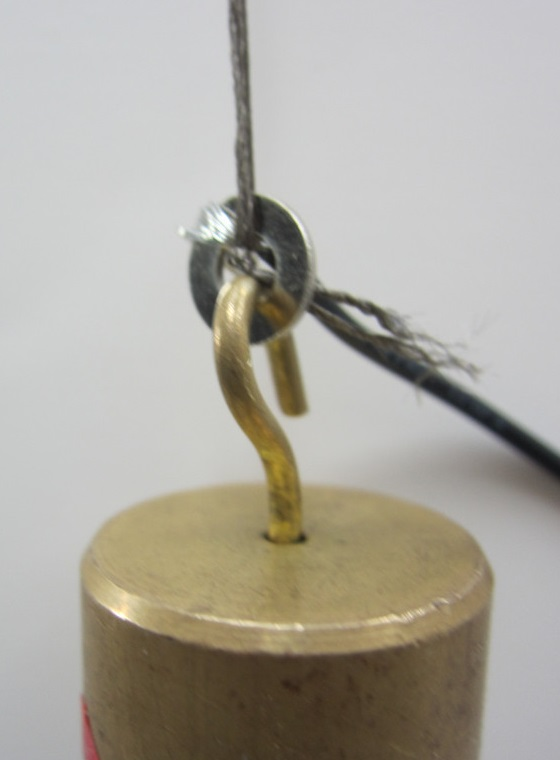
\includegraphics[width=\textwidth]{small_silverSCP_3_v2.jpg}
		\caption{\label{silverSCP_2}}
	\end{subfigure}
	~
	\begin{subfigure}{.45\linewidth}
		\centering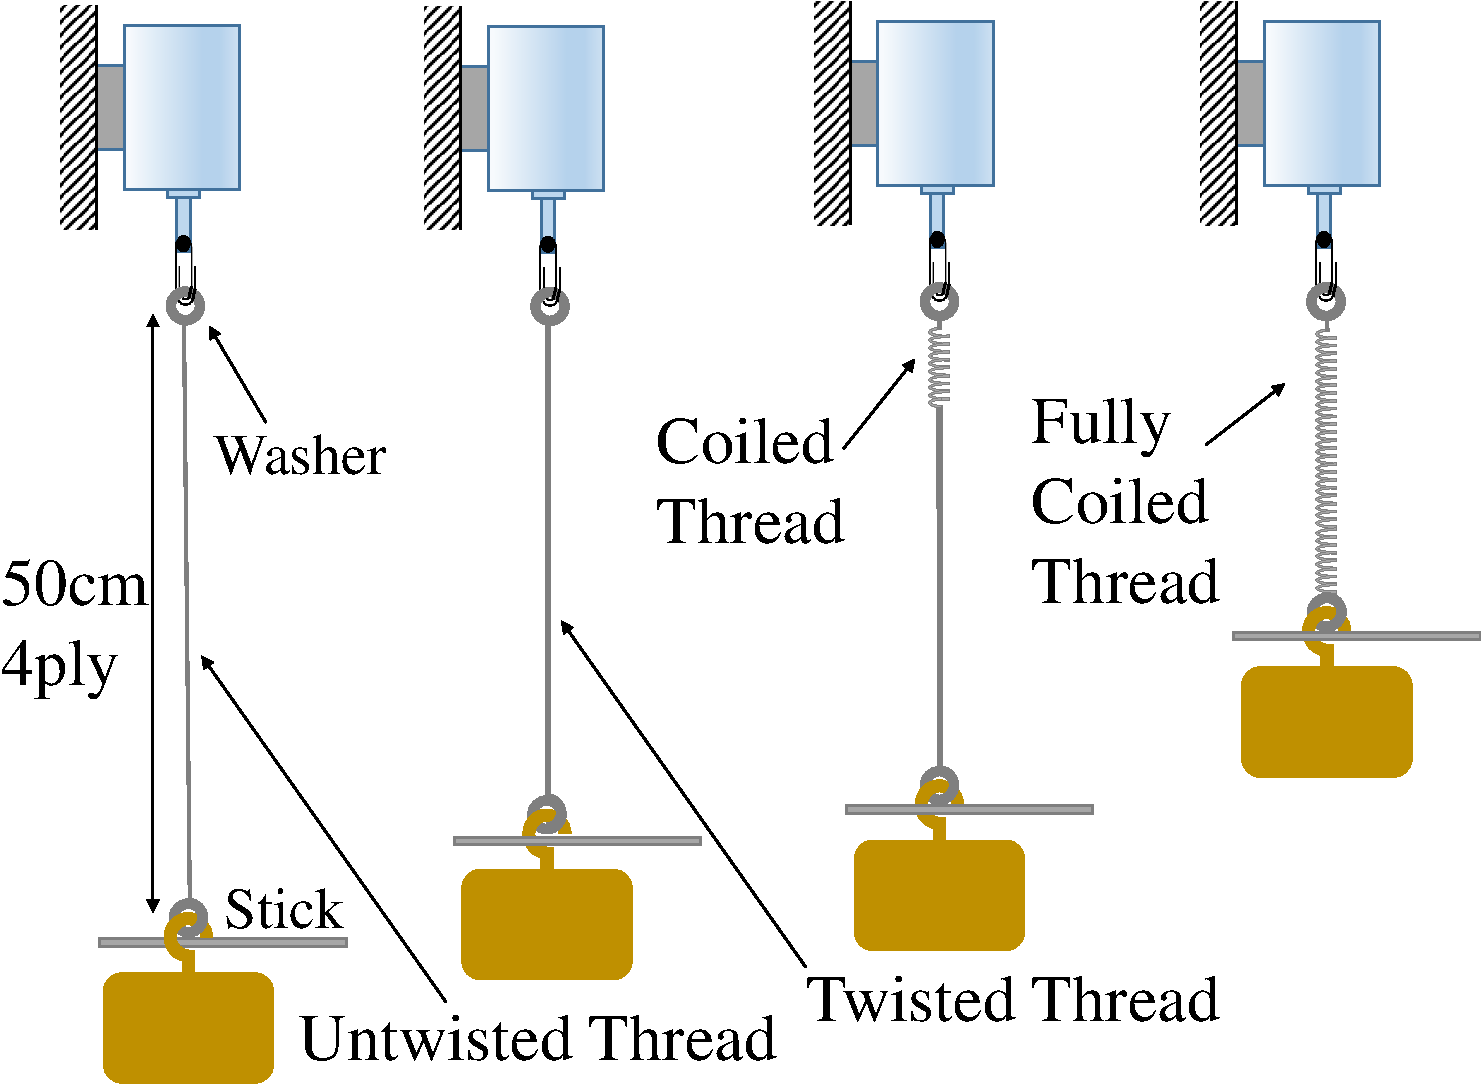
\includegraphics[width=\textwidth]{Fab_illust_v2_crop.pdf}
		\caption{\label{silverSCP_illust}}
	\end{subfigure}
	~
%	\begin{subfigure}{.12\linewidth}
%		\centering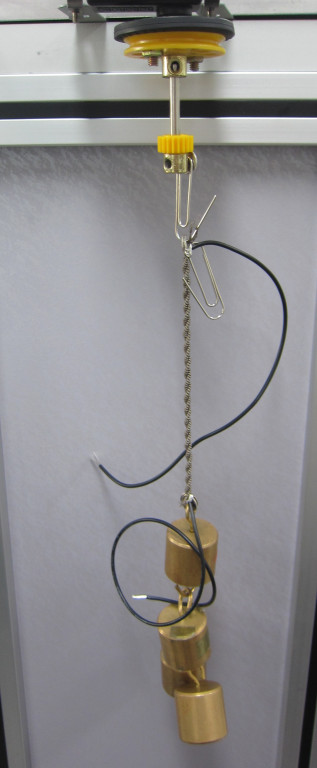
\includegraphics[width=\textwidth]{small_silverSCP_6.jpg}
%		\caption{\label{silverSCP_6}}
%	\end{subfigure}
%	~
	\begin{subfigure}{.15\linewidth}
		\centering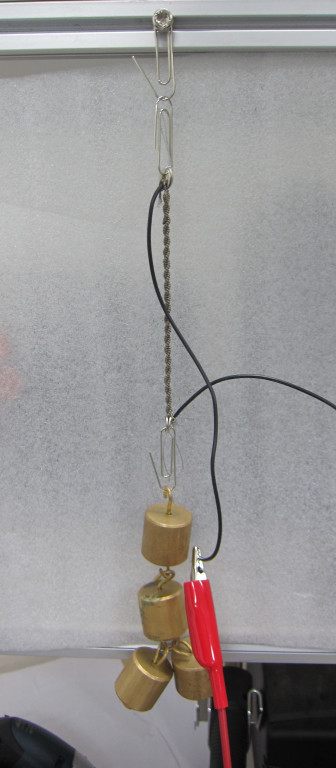
\includegraphics[width=\textwidth]{small_silverSCP_7.jpg}
		\caption{\label{silverSCP_annealing}}
	\end{subfigure}
	\caption[Process of making \scp with silver-painted nylon thread]{Process of making \scp with silver-painted nylon thread.  \subref{silverSCP_2} 4-ply, \SI{50}{\centi\meter} thread bundle's each side was hung on washers. Up side was hung on motor, and down side was hung on \SI{400}{\gram} weight with wire inserted in between washer and thread. \subref{silverSCP_illust} In order to twist thread until it creates coil, down side was fixed with a stick. Two of super coiled polymer was made. Their up side were hung on one clip. Also, their down side were hung on \SI{400}{\gram} weight. Coiled thread's thickness is exaggerated. \subref{silverSCP_annealing} By these processes, \scp was made, which has wire on each side. Finally, they were annealed until length at ambient temperature doesn't get longer.}
	\label{silverSCP_makingof}
\end{figure}

\subsection{Electrical Control of the SCP Artificial Muscles}\label{section_electrical_control}
As discussed in the previous section, the \scp was made with conductive thread in order to electrically control heat speed. Electrical resistance of the \scp was $R=\SI{2.5}{\ohm}$, so the power $P$ was supplied by applying voltage $V=\sqrt{PR}$. The voltage was controlled by MOSFET and PWM generation of Arduino Uno.

In order to implement faster cooling speed of the \scp, a compressed air tank and a solenoid valve were used. The air tank forced air(temperature : equals to  $T_{ambient}$) to flow around the \scp, so we can significantly increase the thermal conductivity of the muscle. Meanwhile, the amount of air flow couldn't be analog controlled. Therefore, by stopping and resuming the flow of air with an appropriate period and ratio, we could control the thermal conductivity of the muscle. This will be discussed at section \ref{section_dynamic} in more details.

\subsection{Physical Measurements of the SCP Artificial Muscles}
Physical properties of the \scps, such as temperature, length, and tension, were measured with various sensors.
\footnote{For the detailed information of sensors, see Table \ref{used_materials}.}
SMD type temperature sensor was used to measure the temperature of the \scps without effecting the specific heat of the \scpnospace.

Also, a slide potentiometer was utilized to measure the linear displacement of the \scpsnospace. However, since it had significant amount of friction, it was only used for the experiments about \scpnospace's characteristics. On the other hand, rotary sensor, which has low frictional torque, was employed to make an \antanospace. 

To measure the tension of the \scpsnospace, a load cell and an amplifier were used.
The load cell played a role in connecting the \scps and the skeleton of the \antanospace.
% As seen as Fig.\ref{anta_loadcell}, load cell played a role of connecting \scp and skeleton of \anta.

\subsection{\ANTAs}
\scps can be easily heated by applying electric current. However, cooling demands more sophisticated procedure. Also, muscles can produce force only when contracting, not for relaxing. This means that \scps can't be directly applied to robots which have to produce force in various positions.
Therefore, we used a principle of antagonism, which is known to be energy-optimal for various tasks \cite{antagonism}.

An \anta was made with two \scpsnospace, which can produce stronger force in two positions within a short time than a single \scpnospace.
First, we made a skeleton of the \anta with 3D printer. (Fig.\ref{3d_assemblies}) Then, non-elongating wire was used to connect stand, muscle, and ball bearing with a rotary sensor inside. A cooling device was also attached to the two \scpsnospace. Lastly, sensors of \anta were connected to Arduino Uno with PCB. (Fig.\ref{anta_overall})

\begin{figure}[t]
	%add desired spacing between images, e. g. ~, \quad, \qquad, \hfill etc. 
	%(or a blank line to force the subfigure onto a new line)
	\centering
	\begin{subfigure}[t]{0.5\textwidth}
		\centering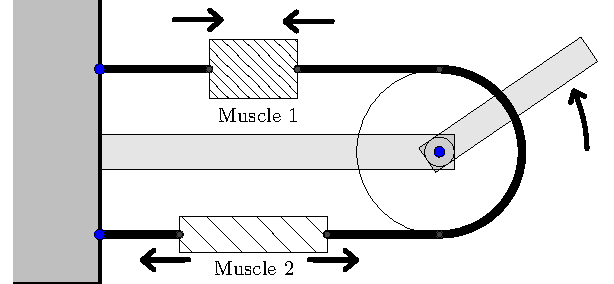
\includegraphics[width=\textwidth]{AntaSchematic_v3.pdf}
		\caption{\label{anta_sch}}
	\end{subfigure}
	~			
	\begin{subfigure}[t]{0.3\textwidth}
		\centering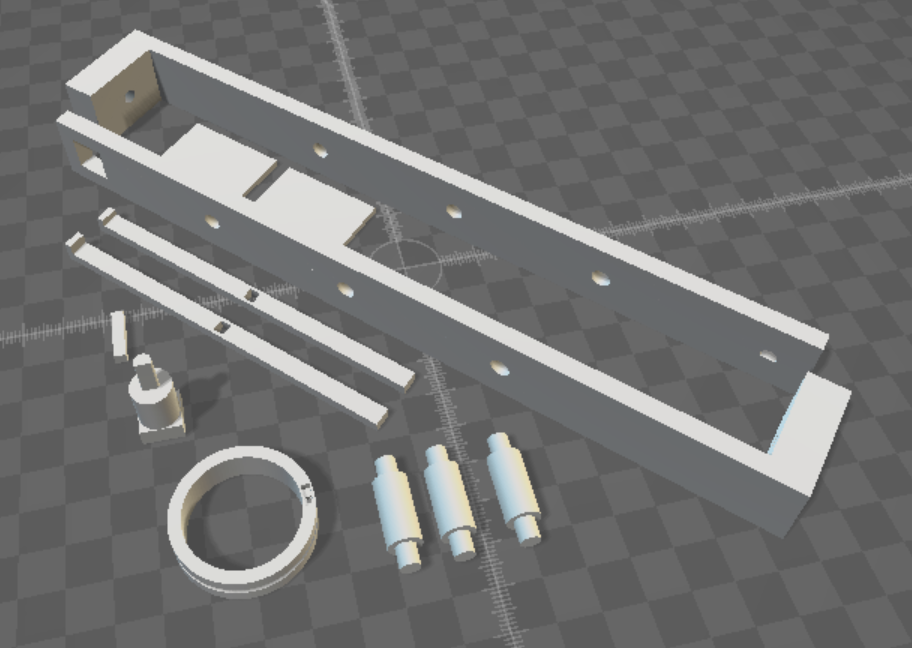
\includegraphics[width=\textwidth]{Anta_3d_assemblies_v2.png}
		\caption{\label{3d_assemblies}}
	\end{subfigure}
	
	\begin{subfigure}[t]{0.81\textwidth}
		\centering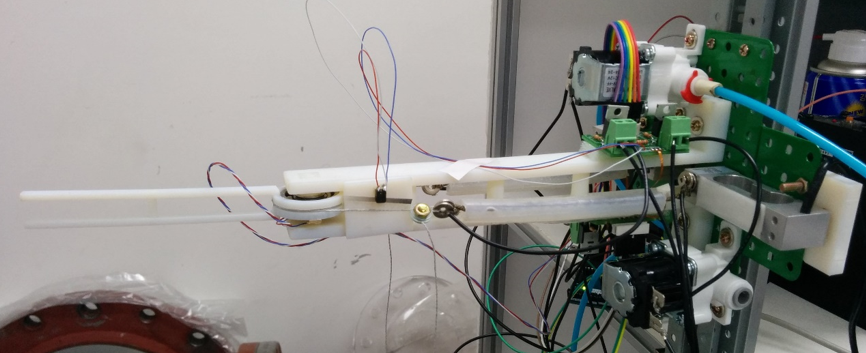
\includegraphics[width=\textwidth]{Anta_overall_v2.png}
		\caption{\label{anta_overall}}
	\end{subfigure}
	
	\caption[An \anta]{\subref{anta_sch} By contracting two \scpnospace s complementarily, we can get same effect of cooling one muscle by heating another. \subref{3d_assemblies} The skeleton of \anta was designed with software(3D Builder, Microsoft) and 3d-printed. \subref{anta_overall} An overall image of \antanospace.}
	\label{anta_design}
\end{figure}

	%\section{Modeling of \scp}\label{section_modeling}
\section{Experiments}\label{section_modeling}
In order to plan a strategy for controlling the tension and length of \scpnospace s, its character must be modeled with mathematical equations. In this section, behavior of \scp was modeled with linear equations and verified by three kinds of experiments. Therefore, equation of \anta was obtained.

\subsection{Modeling of \ANTA}\label{section_thermo_model}
\scp can be expressed as an combination of mechanical model and thermal constant. The correlation between muscle's displacement $x$, temperature $T$, elastic constant $k$, damping constant $b$, thermal constant $c$ and tension $F$ is shown in \eqref{thermo-mechanical_model} \cite{yip}.
\begin{equation} \label{thermo-mechanical_model}
F=k(x-x_0) + b\dot{x}+c(T-T_0)
\end{equation}

Also, by considering Newton's cooling law, the correlation between specific heat $C_{th}$ and thermal conductivity $\lambda$ can be expressed as \eqref{thermo-electrical_model} \cite{yip}.

\begin{equation} \label{thermo-electrical_model}
C_{th}\frac{dT(t)}{dt} = P(t) - \lambda(T(t)-T_{ambient})
\end{equation}

Since \anta is sum of two \scpnospace, the displacement of two \scp is complementarily(Fig.\ref{ModelAnt}). If one of the muscle's displacement is expressed as $\Delta{x}$, another is $-\Delta{x}$. By considering $\Delta{x}=r\theta$ and $\tau=J\ddot{\theta}$, arm's equation of motion is \eqref{EqAnta}, where $r$, $\theta$, $\tau$ and $J$ is radius of arm, rotational displacement, torque and moment of inertia, respectively.

%\begin{align} \label{EqAnta_middle}
%\tau= & \left[  (-k\Delta x-b\dot{\Delta x}+c(T_1-T_0)) \right. \nonumber \\
%& \left. -(k\Delta x+b\dot{\Delta x}+c(T_2-T_0)) \right] r
%\end{align}
%\begin{equation} \label{EqAnta_middle}
%\tau = [-k\Delta x-b\dot{\Delta x}+c(T_1-T_0) - (k\Delta x+b\dot{\Delta x}+c(T_2-T_0))]r
%\end{equation}

\begin{equation} \label{EqAnta}
J\ddot{\theta}+2br^2\dot{\theta}+2kr^2\theta=cr(T_1-T_2)
\end{equation}

\subsection{Aims and Apparatuses}\label{section_aimsappa}
In order to verify and measure constants of model discussed in section \ref{section_thermo_model}, two kinds of experiments were carried out - static, and dynamic experiment. The aims of the experiments are shown below.

\begin{enumerate} 
\item As shown in equation \eqref{thermo-mechanical_model}, to check that muscle's tension changes in respect to length linearly, and to observe a bit of hysteresis caused by $\dot{x}$.
\item To check that muscle's tension changes in respect to temperature linearly.
\item As shown in equation \eqref{thermo-electrical_model}, to check that temperature of muscle changes exponentially and converges to $T_{steady}$ when constant power is supplied.
\item To confirm that $T_{steady}-T_{ambient}$ is proportional to supplied power and get its factor. 
\item To quantify thermal conductivity of muscle when it is cooled with air flow.
%\item To check that muscle damps by damping constant $b$ in \eqref{thermo-mechanical_model}.
\end{enumerate}

In order to achieve first and second aim, we conducted `static experiment' by using following apparatus : An E-shaped holder that holds each side of \scp to maintain constant length which can be customized. (Fig.\ref{static_sch}) Additionally, load cell, temperature sensor, and slide potentiometer was used to measure tension, temperature, and length of \scpnospace, respectively. Also, voltage between muscle was measured to calculate applied power of muscle. These sensors are all connected to NI cRIO-9024 for synchronized real-time data acquisition.

In order to achieve third, fourth, and fifth aim, we conducted `dynamic experiment' by using following apparatus : As shown in Fig.\ref{dynamic_sch}, air can, solenoid valve, and tube which surrounds actuator is connected in sequence. Load was hung on the end in order to prevent muscle becoming loose. 
%\footnote{In this situation, the amount of work used for lifting load is negligible. This will be discussed after calculating $C_{th}$ and $dT/dt$ in section \ref{section_dynamic_results}.} 
Also, temperature sensor was tightly attached to muscle, and connected to Arduino Uno for synchronized real-time data acquisition.


\begin{figure}[t]
	\centering
	\begin{subfigure}[t]{0.2\textwidth}
		\centering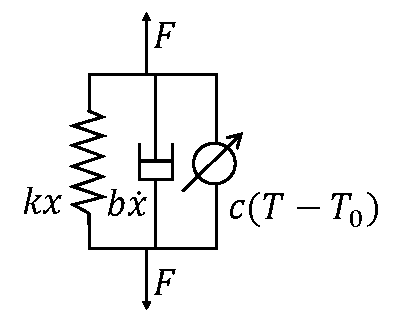
\includegraphics[width=\textwidth]{Model_muscle.pdf}
		\caption{\label{ModelMus}}
	\end{subfigure}
	\begin{subfigure}[t]{0.25\textwidth}
		\centering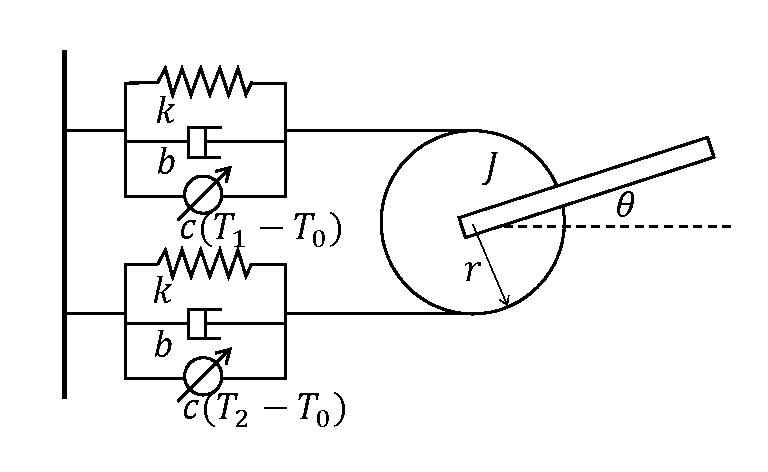
\includegraphics[width=\textwidth]{Model_anta.pdf}
		\caption{\label{ModelAnt}}
	\end{subfigure}
	\begin{subfigure}[t]{0.18\textwidth}
		\centering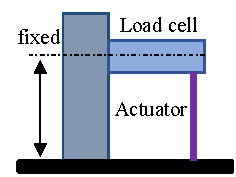
\includegraphics[width=\textwidth]{modeling_static_v2.pdf}
		\caption{\label{static_sch}}
	\end{subfigure}
	\begin{subfigure}[t]{0.18\textwidth}
		\centering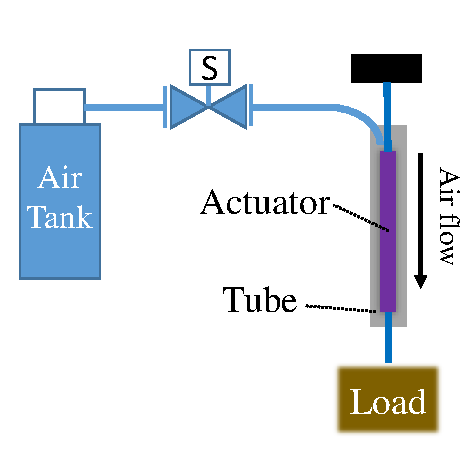
\includegraphics[width=\textwidth]{Static2(v2)_v4.pdf} % An old name of dynamic experiment : static2_v2
		\caption{\label{dynamic_sch}}
	\end{subfigure}
	\caption[Modeling of \scp]{\subref{ModelMus} \scp can be expressed as an combination of a spring, damper, and temperature-dependent system. \subref{ModelAnt} \Anta can be expressed with two complimentary muscles, which change the angular position. \subref{static_sch} Scheme of static experiment. \subref{dynamic_sch} Scheme of dynamic experiment.}
	\label{model+exp_sch}
\end{figure}

\subsection{Static Experiment}
The aim of static experiment was to verify equation \eqref{thermo-mechanical_model} and achieve first and second aim in section \ref{section_aimsappa}. In other words, correlation of \scpnospace's length and tension was investigated at various temperature. 

We can say that muscle have a length $l_{0}$ at ambient temperature with \SI{0}{\newton} tension. Taking $l_{0}$ as standard, we conducted experiments by changing length \SI{15}{\milli\meter} gradually. Also, we used five kinds of voltage - \SI{0}{\volt}, \SI{1.0}{\volt}, \SI{1.8}{\volt}, \SI{2.2}{\volt}, \SI{2.6}{\volt}.

\begin{enumerate}
\item Initial length of \scp was adjusted to $l_0$.
\item We started to apply constant voltage to muscle and waited until muscle's length and temperature becomes steady.
\item When muscle becomes steady, we started recording its physical properties, such as length, tension, temperature, and time.
\item We gradually increased the length of muscle to $l_0+d$.
\item We gradually decreased the length of muscle to $l_0$.
\item End of recording. After cooling to ambient temperature, we repeated 1-5 with other voltage.
\end{enumerate}

Results of static experiment is shown in Fig.\ref{static1_results}. Each of the temperature indicated in legend corresponds to $T_{steady}$. In Fig.\ref{static1_result}, we can observe slight hysteresis. This characteristic graph can be linearly regressed as Fig.\ref{static1_line}. Also, by obtaining force at 10\% strain for each temperature, we can check that force is linearly proportional to $T_{steady}$. By analyzing graph in Fig.\ref{static1_result}, we got values of $k$, $c$ in \eqref{thermo-mechanical_model}.
\begin{equation}
k=\SI{304}{\newton\per\meter}, c=\SI{0.0501}{\newton\per\degreeCelsius} \notag
\end{equation}

\begin{figure}[t]
	\centering
	\begin{subfigure}[t]{0.3\textwidth}
		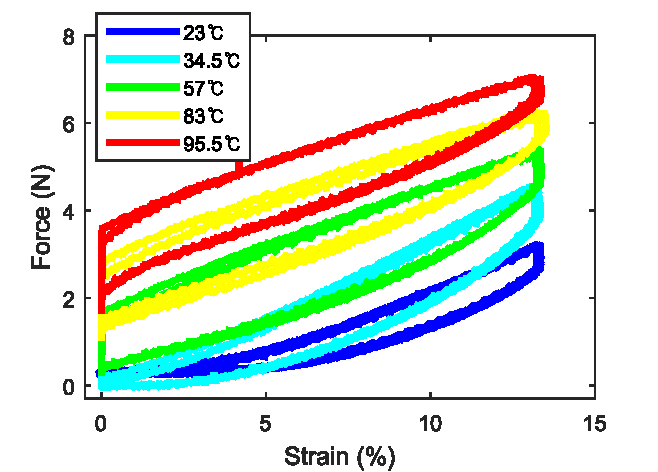
\includegraphics[width=\textwidth]{ForceStrain.pdf}
		\caption{\label{static1_result}}
	\end{subfigure}%
	\begin{subfigure}[t]{0.3\textwidth}
		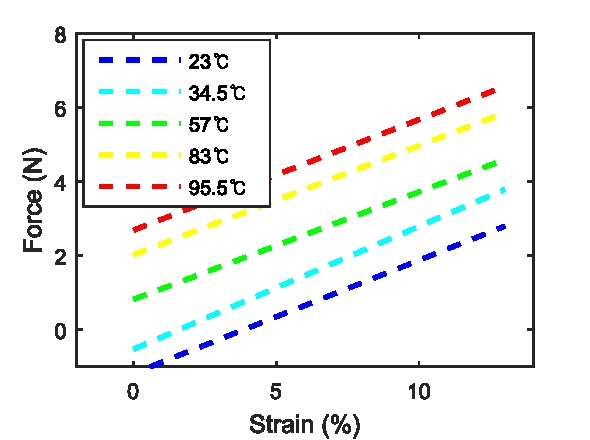
\includegraphics[width=\textwidth]{ForceStrain_line.pdf}
		\caption{\label{static1_line}}
	\end{subfigure}%
	\begin{subfigure}[t]{0.3\textwidth}
		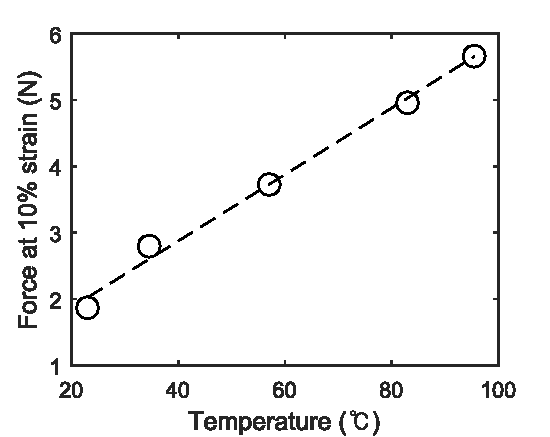
\includegraphics[width=\textwidth]{ForceStrain_dot.pdf}
		\caption{\label{static1_dot}}
	\end{subfigure}
	\caption[Results of static experiment]{\subref{static1_result} Characteristic curves of \scp for various $T_{steady}$. \subref{static1_line} Linear graph of correlation between tension(force) and strain. \subref{static1_dot} Tension is linearly proportional to $T_{steady}$.}
	\label{static1_results}
\end{figure}

\subsection{Dynamic Experiment}\label{section_dynamic} % Important!!
The aim of dynamic experiment was to achieve third to fifth aims in section \ref{section_aimsappa}.
As introduced in section \ref{section_electrical_control}, forced air flow was periodically stopped and resumed to control thermal conductivity of \scpnospace.
This was done by opening the solenoid valve for constant ratio at each period. For example, if we make valve to be opened for \SI{70}{\milli\second} and closed for \SI{30}{\milli\second}, the ratio will be 70\%. From now on, we will call this as `cooling ratio' and use variable name $r$.
 
%With simple assumption, we can simply guess that $\lambda$ will be proportional to $r$, as equation \eqref{dynamic_simple_model}.
%\begin{equation} \label{dynamic_simple_model}
%\lambda = \lambda_{N}+(\lambda_{F}-\lambda_{N})\cdot r (0\leq r \leq 1)
%\end{equation}
%But, the air flow will keep for a short time right after the valve is closed. Therefore, it is expected that thermal conductivity will be constant if ratio is bigger than $r_{c}$. So, we can modify \eqref{dynamic_simple_model} into \eqref{dynamic_complicated}. 
%
%\begin{equation} \label{dynamic_complicated}
%\lambda = \begin{cases}
%\lambda_{N}+(\lambda_{F}-\lambda_{N})\cdot (r/r_{c}) & r_{c1}<r<r_{c2} \\
%\lambda_{F} & r>r_{c2} \\
%\end{cases}
%\end{equation}

The period of opening and closing was \SI{100}{\milli\second}, which was carefully chosen to get best performance. If the period is too long, thermal conductivity of \scp will periodically change. On the other hand, if the period is too short, the solenoid valve won't perform well because it will take minimal time to open the valve. 

We followed a following process to do dynamic experiment. An Arduino code for dynamic experiment is shown in section \ref{code_dynamic}. We used constant voltage - \SI{2.59}{\volt}. Cooling ratio was variously changed, including $0$(Natural cooling, $\lambda_{N}$), and $1$(Complete forced cooling, $\lambda_{F}$). 
\begin{enumerate}
\item When muscle is begin $T=T_{ambient}$, we started recording time and temperature.
\item Constant power was applied until it reaches steady state.
\item After reaching $T=T_{steady}$, power was disconnected and cooling was started. 
\item When muscle's temperature reaches $T=T_{ambient}$ again, we stopped recording. 
\item We repeated process 1-4 with other voltage and cooling ratio.
\end{enumerate}


\begin{figure}[t]
	\centering
	\begin{subfigure}[t]{0.4\linewidth}
		\centering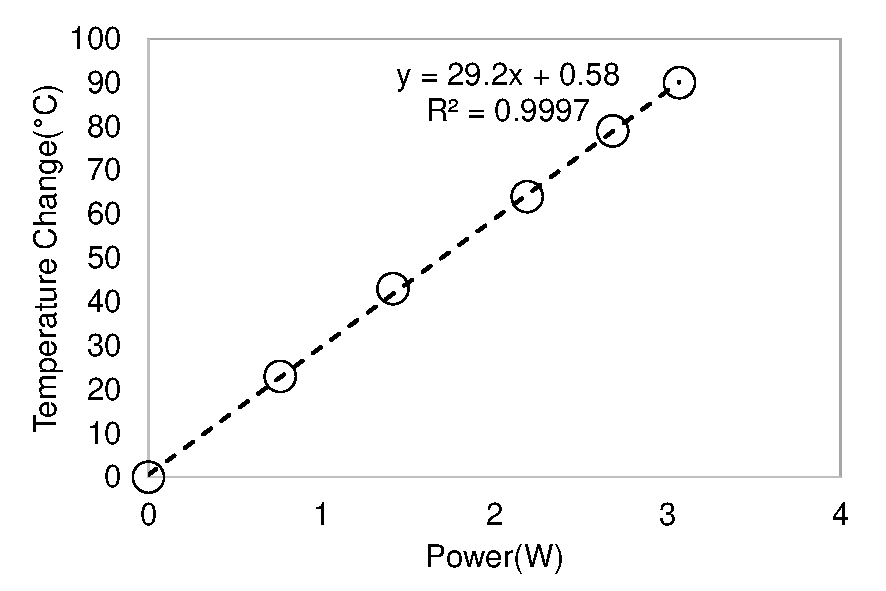
\includegraphics[width=\textwidth]{powerdeltaT-graph_v4.pdf}
		\caption{\label{powerdeltaT}}
	\end{subfigure}%
	\begin{subfigure}[t]{0.4\linewidth}
		\centering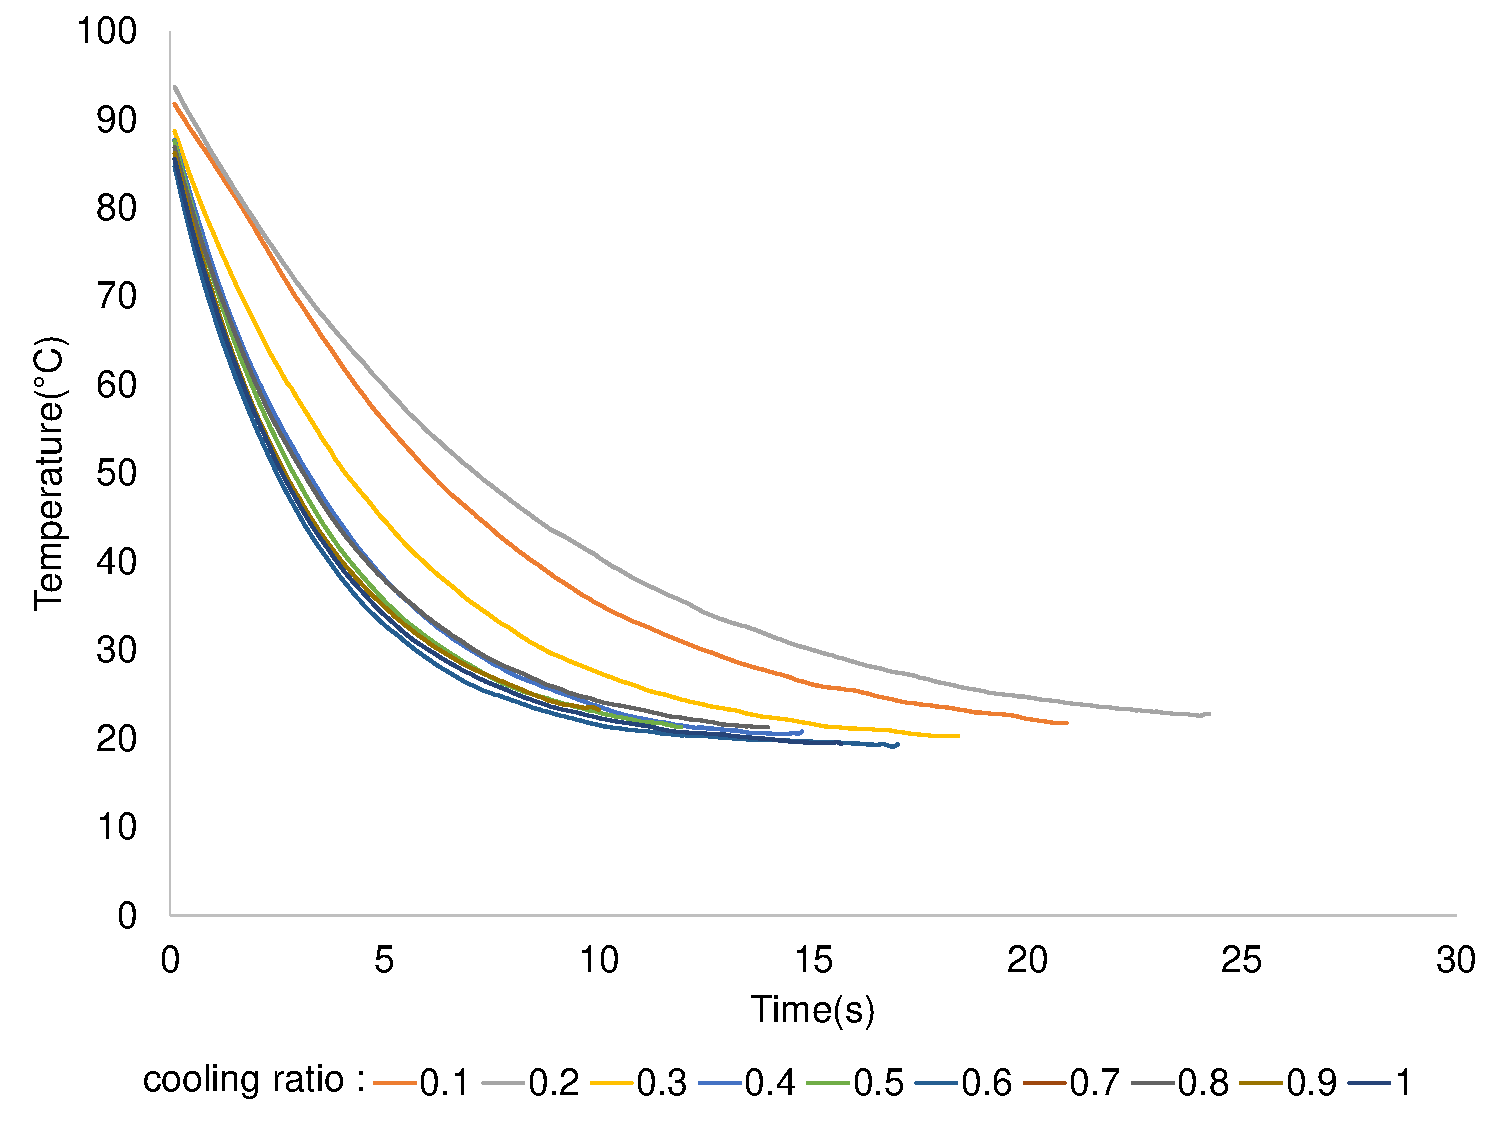
\includegraphics[width=\textwidth]{coolinggraph_v3.pdf}
		\caption{\label{coolinggraph}}
	\end{subfigure}
	\caption[Results of dynamic experiment]{\subref{powerdeltaT} Temperature changes proportionally to power. \subref{coolinggraph} After power was shut down and forced cooling had began, temperature decreased exponentially.}
	\label{result_dynamic}
\end{figure}
%Based on experimental data, we calculated muscle's specific heat $C_{th}$ and thermal conductivity $\lambda$. In detail, we checked that $P$, $\Delta{T}$, $C_{th}$, $\lambda$, and time constant of temperature change $\tau$ satisfies equation \eqref{dynamic_calculation_power} and \eqref{dynamic_calculation_tau}. 

First, by graphing the relation between power $P$ and temperature shift $\Delta{T}=T_{steady}-T_{ambient}$, we could check that they are linearly proportional, as shown in \eqref{dynamic_calculation_power}. The thermal conductivity of \scp was calculated from slope of $\Delta{T} - P$ graph in Fig.\ref{powerdeltaT}.

Also, we could check that temperature of \scp changes exponentially as shown in Fig. \ref{coolinggraph}. This was in line with  \eqref{thermo-electrical_model}.

\begin{equation} \label{dynamic_calculation_power}
P = \lambda\Delta{T}
\end{equation}

Next, by applying \eqref{dynamic_calculation_power} into heating graph, we could get $\lambda_{N}$ according to Fig.\ref{powerdeltaT}. Then, by calculating time constant of heating graph, we could calculate \scp system's specific heat $C_{th}$ with \eqref{dynamic_calculation_tau}.\footnote{This was measured three times, resulting \SI{51.3}{\second}, \SI{54.1}{\second}, \SI{53.0}{\second}. Average was \SI{52.8}{\second}.} 

\begin{equation}
\lambda_{N}=\SI{3.42e-2}{\watt\per\degreeCelsius}, C_{th}=\SI{1.81}{\joule\per\degreeCelsius} \notag
\end{equation}

%Meanwhile, as predicted in \eqref{dynamic_complicated}, if $r<0.6$, then $\lambda\propto r$. Else, $\lambda$ was constant, same with $\lambda_{F}$ when $r=1.0$.

Now, we have value of $C_{th}$, so thermal conductivity can be obtained by using \eqref{dynamic_calculation_tau}. Analysis for each cooling graphs is shown in Fig.\ref{analysis_dynamic}.

\begin{equation} \label{dynamic_calculation_tau}
\lambda = \frac{C_{th}}{\tau}
\end{equation}

\begin{figure}[t]
	\begin{subfigure}[t]{0.52\linewidth}
		\centering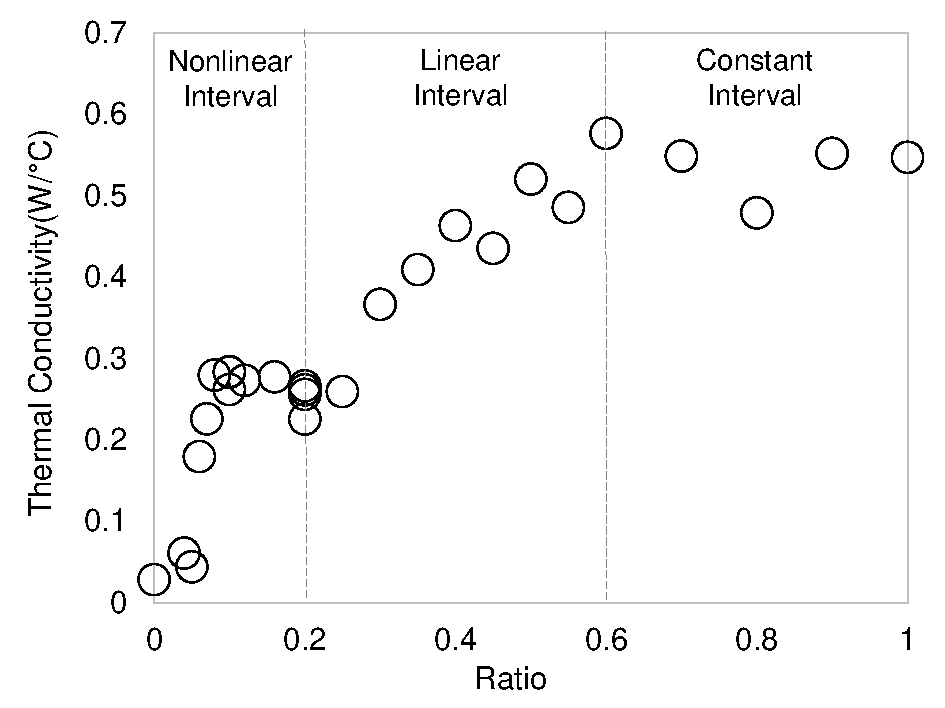
\includegraphics[width=\textwidth]{intervals_v3.pdf}
		\caption{\label{dynamic_proportional}}
	\end{subfigure}%
	\begin{subfigure}[t]{0.39\linewidth}
		\centering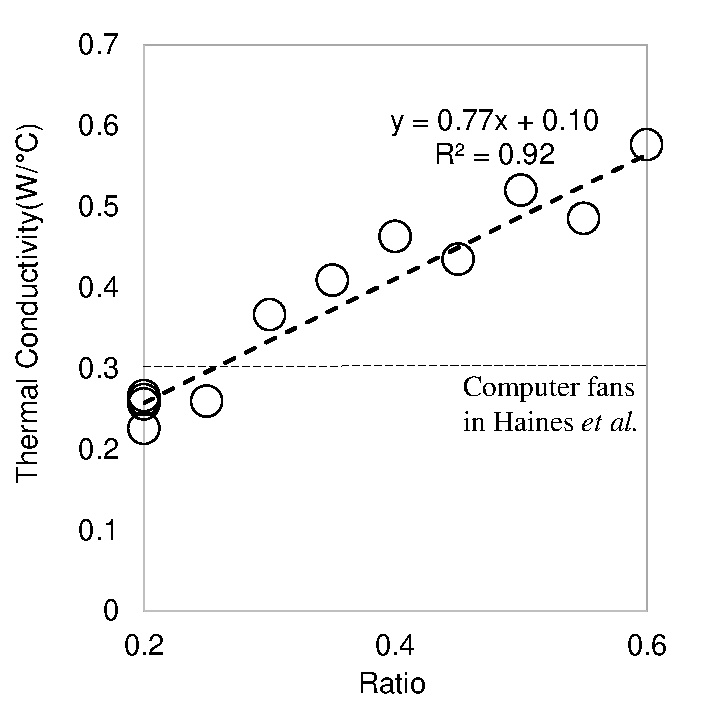
\includegraphics[width=\textwidth]{linear_interval_v4.pdf}
		\caption{\label{linear_interval}}
	\end{subfigure}
	\caption[Analysis of dynamic experiment]{\subref{dynamic_proportional} $\lambda$ was linearly proportional to cooling ratio $r$ when $0.2<r<0.6$.  \subref{linear_interval} $\lambda$ can be calculated with equation \eqref{lambda_control}.}
	\label{analysis_dynamic}
\end{figure}

In Fig.\ref{dynamic_proportional}, we could observe that thermal conductivity in function of $r$ can be divided into three parts - nonlinear, linear, and constant interval. If $r<0.2$, $\lambda$ rapidly increased near $r=0.1$. Also, $\lambda$ doesn't increased anymore if $r>0.6$, {\it i.e.} $\lambda = \lambda_{F}$. Therefore, the linear interval was chosen for \Apcnospace. The thermal conductivity in controllable(linear) interval was higher than cooling by computer fans, which were used by Haines \etalspace and determined to be $\lambda_{fan}=\SI{0.30}{\watt\per\degreeCelsius}$.

\begin{equation} \label{lambda_control}
\lambda = 0.77\cdot r + 0.10 (\si{\watt\per\degreeCelsius}), 0.2\leq r \leq 0.6
\end{equation}


%Meanwhile, we have to justify the approximation used in section \ref{section_dynamic_appa}. 
Meanwhile, we have to check that the load used in dynamic experiment doesn't effected muscle's thermal power. % (?)
Total electrical power of muscle is about $(\SI{1.0}{\volt})^2/(\SI{2.5}{\ohm})=\SI{0.4}{\watt}$, cooling speed is about $\SI{1.39}{\joule\per\degreeCelsius} \cdot \SI{1}{\degreeCelsius\per\second}=\SI{1.39}{\watt}$ while gravitational power is about  $\SI{0.4}{\kilo\gram} \cdot  \SI{9.8}{\meter\per\second\square} \cdot \SI{0.001}{\meter\per\second}=\SI{0.004}{\watt}$. So we can conclude that load didn't affected on measurement of muscle's thermal properties.




	\section{Control}
In the previous section, mathematical modeling of \scp was discussed. In this section, control strategies and their results are shown. Based on models in section \ref{section_modeling}, \anta was controlled to follow desired position, which is a function of time. We will now call this as \apcnospace.

\subsection{Basic Strategy of \APC}
By assuming that $\ddot{\theta}$ and $\dot{\theta}$ is small enough, we can get correlation between $\theta$ and $T_{1}$, $T_{2}$ from \eqref{EqAnta} as \eqref{simple_assume}.
\begin{equation} \label{simple_assume}
\theta = \frac{c}{2kr}(T_{1}-T_{2})
\end{equation}
By multiplying Laplace transformation of \eqref{thermo-electrical_model} and \eqref{simple_assume}, we can get transfer function of $P$ and $\theta$ as \eqref{apc_transfer}.

\begin{equation} \label{apc_transfer}
\frac{\theta(s)}{P(s)} = \frac{c/2kr}{C_{th}s+\lambda}
\end{equation}

Therefore, process of controlling $\theta$ into $\theta_{ref}$ by applying constant power can be shown as block diagram in Fig.\ref{AntaControl_constant}. 

In this situation, $K_{\theta,P}$ is constant. By applying constant power to only one of the muscle, $\theta$ at steady state was measured. Linear fitting of Fig.\ref{KthetaP} gives us following constant.

\begin{equation}
K_{\theta,P} = \SI{0.185}{\watt\per\degree} \notag
\end{equation}

For fast and precise control, lead compensator was added and feedback, feedforward was applied, as can be seen in Fig.\ref{position_open_loop}, \ref{position_closed_loop}.

\begin{figure}[b]
	\centering
	\begin{minipage}{0.35\textwidth}
		\begin{subfigure}{\linewidth}
			\centering
			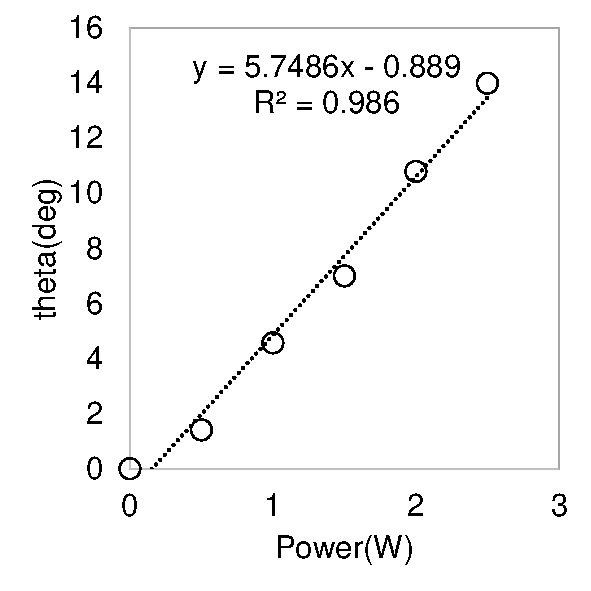
\includegraphics[width=\linewidth]{K_theta_P_v3.pdf}
			\caption{\label{KthetaP}}
		\end{subfigure}
	\end{minipage}%
	\begin{minipage}{0.6\textwidth}
		\begin{subfigure}{\linewidth}
			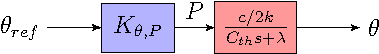
\includegraphics[width=\linewidth]{Diagram(v4)_position_constant.pdf}
			\caption{\label{AntaControl_constant}}
		\end{subfigure}
		
		\begin{subfigure}{\linewidth}
			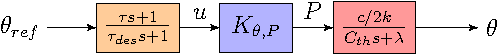
\includegraphics[width=\linewidth]{Diagram(v4)_position_openloop.pdf}
			\caption{\label{position_open_loop}}
		\end{subfigure}
		
		\begin{subfigure}{\linewidth}
			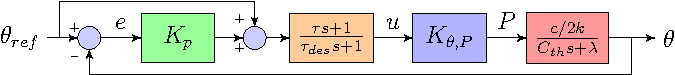
\includegraphics[width=\linewidth]{Diagram(v4)_position_feedback.pdf}
			\caption{\label{position_closed_loop}}
		\end{subfigure}
	\end{minipage}
	\caption[Block diagrams for \apc]{\subref{KthetaP} There's a linear relationship between applied power and $\theta$ at steady state. \subref{AntaControl_constant} Process of obtaining desired angle with constant power. \subref{position_open_loop} Process of \apc including lead compensator. \subref{position_closed_loop} Process of \apc including feedback and feedforward.}
	\label{anta_position_diagrams}
\end{figure}


\subsection{Antagonistic Position Control Strategy for Making Sin Wave Motion}
In this section, we aim to make a simple sin wave motion of \anta as \eqref{theta_ref}. By doing this, we could check the possibility of \apc for any complicated motion. Basically, according to the equation \eqref{simple_assume}, we can increase $\theta$ by heating muscle 1 and decrease $\theta$ by heating muscle 2. Therefore, we used a strategy shown in Table.\ref{table_apc_basic}
%By assuming that $\ddot{\theta}$ and $\dot{\theta}$ is small enough, \eqref{EqAnta} can be approximated into \eqref{EqAngleTempDiff}.

%\begin{equation}\label{EqAngleTempDiff}
%\theta=\frac{c}{2kr}(T_1-T_2)
%\end{equation}



\begin{equation}\label{theta_ref}
\theta_{ref}(t)=(\SI{9}{\degree})\sin(2\pi 0.025t)
\end{equation}

\begin{table}[b]
	\caption{Basic strategy of \apc for making sin wave motion.}
	\label{table_apc_basic}
	\begin{center}
		\begin{tabular}{c||c|c|c|c}
			\hline
			Time(s) & 0-10 & 10-20 & 20-30 & 30-40 \\
			\hline
			Muscle 1 & Heat & Keep & Keep & Heat \\
			Muscle 2 & Keep & Heat & Heat & Keep \\
			\hline
			$\theta$ & increase & decrease & decrease & increase \\
			\hline
		\end{tabular}
	\end{center}
\end{table}

Since the Laplace transformation of \eqref{theta_ref} is too complicated, we used an approximation shown in \eqref{theta_ref_approx} by dividing \eqref{theta_ref} into 12 steps. In this case, demanded power can be calculated as \eqref{power_derived}. ($n=12$)
\footnote{In equation \eqref{power_derived}, $\theta_{ref,pre}$ is value of $\theta_{ref}$ in previous step. Also, $t$ is elapsed time after starting new step.}. 
\footnote{$U(t)$ is unitary step function.}
An Arduino code for \apc is given in appendix \ref{code_dynamic}.
\begin{equation} \label{theta_ref_approx}
\begin{aligned} 
%\theta_{ref}(t) = \sum_{i=0}^{n-1}{(\theta_{ref,i+1}-\theta_{ref,i})U(t-i\Delta T)} 
\theta_{ref}(t) & = \sum_{i=0}^{n-1}{(\theta_{ref,i+1}-\theta_{ref,i})U(t-i\Delta T)} \\
& = \sum_{i=0}^{n-1}{(\sin{\frac{2(i+1)\pi}{n}}-\sin{\frac{2i\pi}{n}})U(t-40\frac{i}{n})} \\
\end{aligned}
\end{equation}

\begin{equation} \label{power_derived}
P(t)=\theta_{ref}K_{\theta,P}(1+(\frac{\theta_{ref}-\theta_{ref,pre}}{\theta_{ref}})(\frac{\tau}{\tau_{des}}-1)e^{-\frac{t}{\tau_{des}}})
\end{equation}

 %Through these steps, we can do \apc as a sin wave form.

\begin{figure}[t]
	\centering
	\begin{subfigure}[t]{0.44\textwidth}
		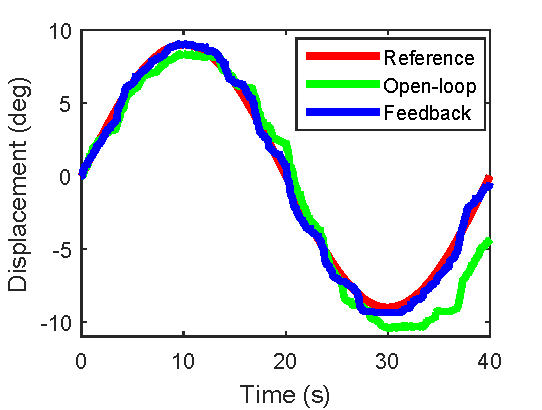
\includegraphics[width=\textwidth]{SinWave.pdf}
		\caption{\label{positionControl_sin}}
	\end{subfigure}%
	\begin{subfigure}[t]{0.50\textwidth}
		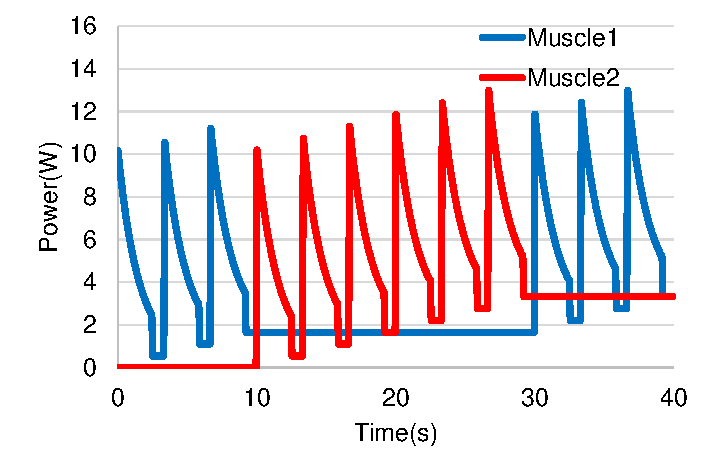
\includegraphics[width=\textwidth]{Openloop_power_graph_v2.pdf}
		\caption{\label{positionControl_sin_power}}
	\end{subfigure}
	\caption[\Apc by only heating]{\subref{positionControl_sin} Measured arm's angular position in function of time. Feedback control had smaller error than open-loop control. \subref{positionControl_sin_power} Used power of each \scpnospace s(Open loop)}
	\label{positionControl}
\end{figure}

\clearpage

\subsection{Sustainable Antagonistic Position Control Strategy with Cooling Method}\label{section_simulation}
In previous section, the method for making sin wave motion was discussed. But since the temperature of muscle in initial state and final state is significantly different, it won't be sustainable because the temperature will keep going up. Therefore, we need to make the temperature of initial state and final state to be same. This can be done by cooling the muscle during last 1/4 period of sin wave, as shown in Table \ref{table_apc_sustain}.

\begin{table}[b]
	\caption{Sustainable \apc strategy by using cooling}
	\label{table_apc_sustain}
	\begin{center}
		\begin{tabular}{c||c|c|c|c|c|c}
			\hline
			Time(s) & 0 & 0-10 & 10-20 & 20-30 & 30-40 & 40 \\
			\hline
			Muscle 1 & $T_0$ & Heat & Keep & Keep & Weakly Cool & $T_0$ \\
			Muscle 2 & $T_0$ & Keep & Heat & Heat & Strongly Cool & $T_0$ \\
			\hline
			$\theta$ & $0^{\circ}$ & increase & decrease & decrease & increase & $0^{\circ}$ \\
			\hline
		\end{tabular}
	\end{center}
\end{table}

\tocless \subsubsection{Demonstration - Two Period Sin Wave}
First, we demonstrated open-loop control of cooling speed. Two-period sin wave control was done, and cooling was done in during $t=$\SI{40}{\second} - \SI{50}{\second}.\footnote{This slightly differs from Table \ref{table_apc_sustain}.} In order to cool as much as possible, muscle 2 was cooled for all time, and muscle 1 was `weakly' cooled by repeatedly opening and closing the solenoid valve. As a result, we got an rms error 26.6\% for open-loop control, and 6.7\% for closed-loop control.(Fig.\ref{sustain_demo})

%After the demonstration, we concluded that an appropriate time for cooling will be \SI{30}{\second}-\SI{40}{\second}, not \SI{40}{\second} - \SI{50}{\second}. It is because 
\begin{figure}[t]
	\centering
	\begin{subfigure}[t]{0.47\textwidth}
		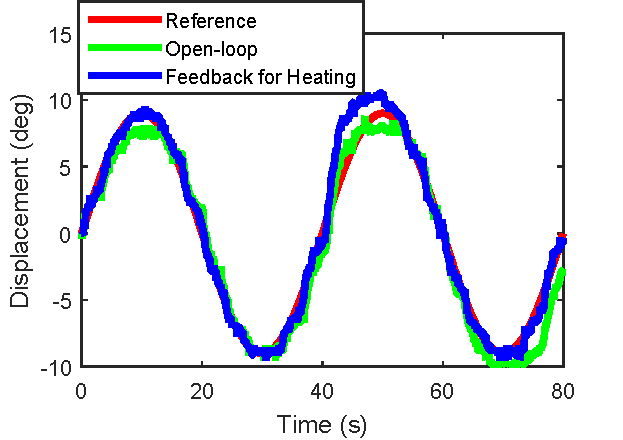
\includegraphics[width=\textwidth]{SinWave_cooling.pdf}
		\caption{\label{SinWave_cooling}}
	\end{subfigure}
	~
	\begin{subfigure}[t]{0.46\textwidth}
		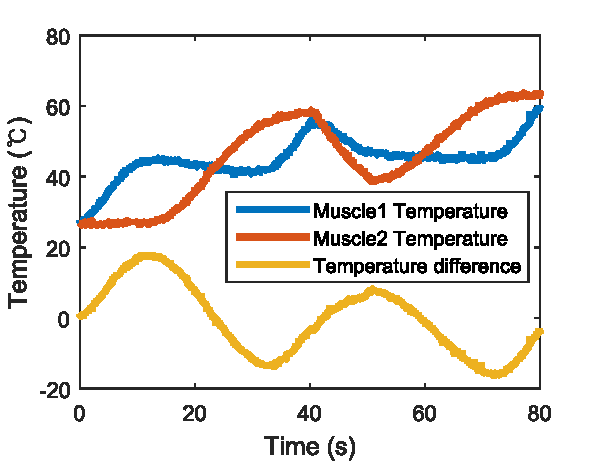
\includegraphics[width=\textwidth]{SinWaveC_T.pdf}
		\caption{\label{Sinwave_C_T}}
	\end{subfigure}
	\caption[Sustainable open-loop \apc demonstration]{\subref{SinWave_cooling} Arm's angle in function of time. \subref{Sinwave_C_T} Temperature of two muscles in function of time. We checked that sustainable \apc is possible by cooling for some time.}
	\label{sustain_demo}
\end{figure}

\tocless \subsubsection{Simulation - Feedback Control of Thermal Conductivity}


Integrating \eqref{dynamic_calculation_tau} and \eqref{lambda_control}, we can get \eqref{tau_modification}.
\begin{equation} \label{tau_modification} 
\begin{aligned} 
\tau & = \frac{C_{th}}{\lambda} \\
& = \frac{1.81}{0.77\cdot r + 0.10} \\ 
\end{aligned}
\end{equation}

Also, time derivative of \eqref{simple_assume} and \eqref{theta_ref}, we can get \eqref{theta_diff} where $t$ is time elapsed since $t=\SI{30}{\second}$.

\begin{equation} \label{theta_diff}
\begin{aligned} 
\frac{d\theta}{dt} & = \frac{c}{2kr}\cdot\frac{d}{dt}(T_{1}-T_{2}) \\
& = 9^{\circ}(2\pi\cdot 0.025)\sin{2\pi\cdot 0.025t} 
\end{aligned}
\end{equation}


What we have to do is decreasing $(T_{1}+T_{2})/2$, so we will use equation \eqref{diff_t1+t2}. Constant $\alpha$ was carefully determined by many times of simulations.
\begin{equation} \label{diff_t1+t2}
\frac{d}{dt}(T_{1}+T_{2}) = -\alpha(T_{1}+T_{2}-2T_{ambient})
\end{equation}

Therefore, by using \eqref{thermo-electrical_model} for each muscles, we can calculate needed $\lambda_{1}$, $\lambda_{2}$. The block diagram which represents feedback control of thermal conductivities is shown in Fig.\ref{diagram_sustainable}.

\begin{figure}[t]
	\centering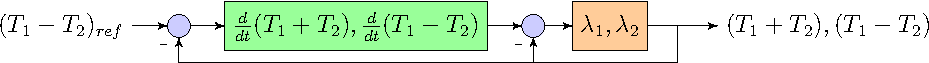
\includegraphics[width=\textwidth]{Diagram(v4)_sustainable.pdf}
	\caption{Block diagram for sustainable \apcnospace.}
	\label{diagram_sustainable}
\end{figure}

To make sustainable \apc possible, $\lambda$ must be between $\SI{0.25}{\watt\per\degreeCelsius}$ and $\SI{0.60}{\watt\per\degreeCelsius}$ for all time, according to \eqref{lambda_control}. Therefore, possibility of this control strategy was verified by thermal simulation.
%We can guess that $\lambda_{1}$ have to decrease and $\lambda_{2}$ have to increase. 

During $t=\SI{30}{\second}$ $t=\SI{40}{\second}$, $\lambda_{1}$ have to decrease and $\lambda_{2}$ have to increase. Therefore, we need to make $\lambda_{1}$ and $\lambda_{2}$ to reach its limit as late as possible. This is determined by constant $\alpha$. 
In Fig.\ref{Sinwave_C_T}, we could observe that two of the muscles' average temperature has increased approximately  \SI{30}{\degreeCelsius}. This means that we have to cool down the average temperature at least \SI{30}{\degreeCelsius}. 

Simulation was carefully done by applying \eqref{thermo-electrical_model} and \eqref{EqAnta}, using the constants we got in section \ref{section_modeling}. The differential equation was numerically solved with 4th Runge-Kutta method.
Through many times of simulations, we had concluded that $\alpha = 0.23$ is the best. The result of simulation with this value is shown in Fig.\ref{cool_simulation}. In Fig.\ref{cool_control_T}, we can observe that average temperature of two muscles had decreased over \SI{30}{\degreeCelsius}, before reaching limit thermal conductivity as shown in Fig.\ref{cool_control_lambda}. Finally, we can conclude that feedback cooling control is possible.

\begin{figure}[t]
	\centering
	\begin{subfigure}[t]{0.45\textwidth}
		\centering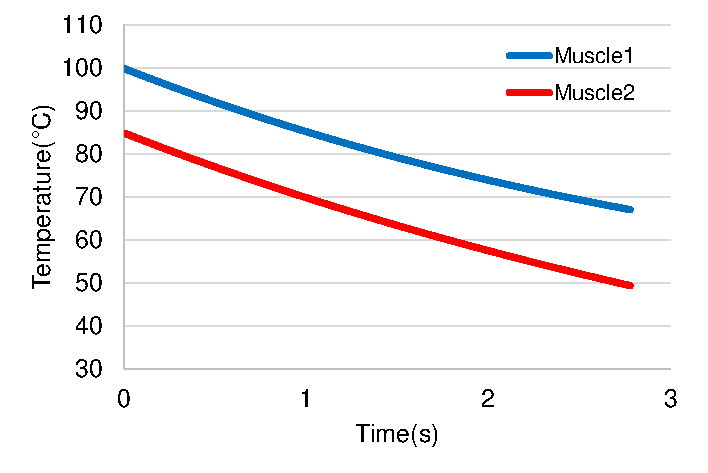
\includegraphics[width=\textwidth]{cool_control_T_v2.pdf}
		\caption{\label{cool_control_T}}
	\end{subfigure}%
	\begin{subfigure}[t]{0.45\textwidth}
		\centering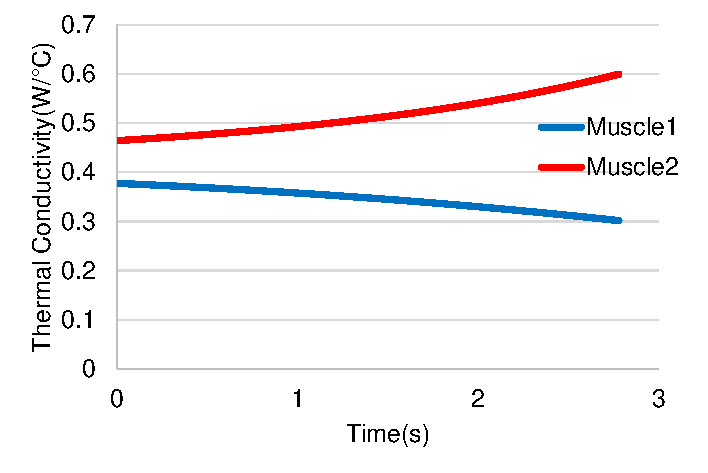
\includegraphics[width=\textwidth]{cool_control_lambda_v2.pdf}
		\caption{\label{cool_control_lambda}}
	\end{subfigure}
	\caption[Sustainable closed-loop \apc simulation]{\subref{cool_control_T} Temperature of two muscles in function of time after $t=\SI{30}{\second}$. \subref{cool_control_lambda} Thermal conductivity of two muscles in function of time. }
	\label{cool_simulation}
\end{figure}





	% Next Section (e.g. Experiment, Linear theory, etc...) 
	% 이외에도 추가로 section마다 파일을 sub 폴더 안에 넣고 여기에서 
	% include 해주면 됩니다.
	% 예시 : methodology.tex을 sub 폴더안에 저장, 이 자리에 
	% \include{sub/methodology} 와 같이 작성
	%%%% 주의
	%%%% 파일이 나뉠 때마다 자동으로 페이지넘김(\clearpage)가 됩니다. 
	%%%% 따라서 subsection을 나누는 용도로는 사용하지 마십시오.
	%%%% \include{sub/experiment} 와 같이...
	
	
	\section{Conclusion}
Various investigations for the method of \scpnospace's efficient control have been done by preceding researches \cite{haines,mirvakili,yip}. %1
However, these studies haven't established efficient methods for cooling \scpnospace. %2
%This could be solved by using antagonism, but yet not sustainable.
In this study, \antas were made to perform fast response of displacement on two sides, but they were not yet sustainable. Thus, we tested the performance of the cooling method with a compressed air can, to demonstrate the sustainable \apcnospace, and proved it through simulations of thermodynamical models. %3

We found that the thermal conductivity of \scp can be feedback controlled by repeating opening and closing of the solenoid valve in variable ratios for a certain period of time. %4
This is done by using compressed air, which is known to be natural method in operating temperature, along with water cooling \cite{madden}.
Also, this method showed higher thermal conductivity than that of cooling by computer fans \cite{yip}.
Therefore, this study has been extending the achievement of Yip \etal, proving that \apc can be highly sustainable.

Most notably, this is the first study to make thermal conductivity feedback controlled. This could be done by extraordinary idea - opening and closing of the  solenoid valve repeatedly.
%Since hysteresis of \scp is known to be lower at high temperature \cite{moretti}, 
However, some limitations on this study are worth noting. 
%Required temperature for feedback cooling was too high, which is not energy-efficient.
Compressed air cans had to be replaced frequently because the pressure of them wasn't constant enough. 
Also, solenoid valve's operating sound and vibration were too big to be applied into real robots.
%Future work should therefore try the forced air cooling through tube with big capacity such as Helium tank. 
Further research should therefore establish efficient, mobile cooling methods and or devices for \scps with larger capacity. 
Extra equipments such as portable air compressors can be used as cooling device.
%This will also provide higher thermal conductivity since Helium have smaller molecular mass than atmosphere.


%% Tank 보다는 Can 을 사용함으로써 휴대 가능하게 함
%% 하지만 Can 이라서 빨리 소진되는 경향이 있기는 함

% 'Electrical heating combined with compressed air or water for cooling are natural choices in the operating room. : Madden2015 : `Twisted Lines % Conclusion
	
	
\clearpage  %%% Appendix를 새 페이지에서 시작
\appendix
\renewcommand{\thesection}{\Alph{section}} %%% TOC에 appendix numbering 재설정
\renewcommand{\thesubsection}{\arabic{subsection}}
\renewcommand{\thesubsubsection}{\arabic{subsubsection}}
\titleformat{\section}[hang] {\normalfont\LARGE\bfseries}{\Alph{section}.}{1em}{} %%% Appendix section title의 재설정
\titleformat{\subsection}[hang] {\normalfont\Large\bfseries}{\Alph{section}.\arabic{subsection}.}{1em}{}
\titleformat{\subsubsection}[hang] {\normalfont\bfseries}{\Alph{section}.\arabic{subsection}.\arabic{subsubsection}.}{1em}{}
\renewcommand{\theequation}{\thesection.\arabic{equation}} %%% Appendix equation numbering 의 재설정
\renewcommand{\thefigure}{\thesection-\arabic{figure}} %%% Appendix figure numbering 의 재설정
\renewcommand{\thetable}{\thesection-\arabic{table}} %%% Appendix table numbering 의 재설정
\setcounter{equation}{0} %%% Appendix equation starting number의 초기화
\setcounter{figure}{0} %%% Appendix figure starting number의 초기화
\setcounter{table}{0} %%% Appendix table starting number의 초기화


\begin{landscape}
\section{List of the Utilized Materials}
\begin{table}[h]
	\caption[List of the Utilized Materials.]{List of the utilized materials. DM : \url{devicemart.co.kr} / EP : \url{eleparts.co.kr}}
	\label{used_materials}
	\begin{center}
		\begin{tabular}{m{0.28\textwidth}||m{0.2\textwidth}|m{0.25\textwidth}|m{0.35\textwidth}|m{0.2\textwidth}}
			\hline
			Item & Name & Manufacturer & Note & Website \\
			\hline
			
			
			\hline
			\multicolumn{5}{l}{Sensors} \\ \hline
			Temperature sensor & \small{TC1047AVNB} & Microchip & \small{\SI{-40}{\degreeCelsius}-\SI{125}{\degreeCelsius}} & DM/\url{10846} \\
			\hline
			Rotary sensor & \small{SV01A103 AEA01B00} & Murata & Frictional torque : \SI{2}{\milli\newton\meter} & EP/\url{EPX47RBF} \\
			\hline
			Slide potentiometer & PTA2043 & Bourns & Max displacement : \SI{20}{\milli\meter} & \url{mouser.com} \\
			\hline
			Load cell & CB1A & Dacell & CAPA : \SI{3}{\kg f} & \url{dacell.com} \\
			\hline
			Amplifier & DN-AM100 & Dacell & Amp X100 - X1500 & \url{dacell.com} \\
			\hline
			Data acquisition system & \small{NI cRIO-9024} & \small{National Instruments} & Maximum voltage : \SI{10}{\volt} & \url{ni.com} \\
			\hline
			
			
			\hline
			\multicolumn{5}{l}{Actuating system} \\ \hline
			Conductive nylon thread & \small{Conductive Yarn} & Shieldex & Size 92 & \url{jameco.com} \\
			\hline
			{\bf Compressed air can} & Dr.99 & \small{BEX Intercorporation} & Nonflammable & DM/\url{9090} \\
			\hline
			{\bf Solenoid valve} & HSV-FF & StormTec & High-pressure, DC 12V & \url{stormtec.co.kr} \\
			\hline
			{\bf Computer fan} & \small{DF0601512SEU2F} & Cool Flow & \SI{12}{\volt}, Size : 60x60x15 \si{\milli\meter} & DM/\url{1078145}\\
			\hline
			
			
			\hline
			\multicolumn{5}{l}{\Anta} \\ \hline
			MOSFET & IRFZ44N & {\small International Rectifier} & Maximum current : \SI{35}{\ampere} & DM/\url{1477} \\
			\hline
			PCB & Sample PCB & Devicemart & custom service & DM/\url{33755} \\
			\hline
			Ball bearing & 6000OPEN & KBC & OD / ID : \SI{26}{\milli\meter}, \SI{10}{\milli\meter} & EP/\url{EPX38VPJ} \\
			\hline
			Arduino Uno & Arduino Uno & arduino.cc & Certified & \\
			\hline
		\end{tabular}
	\end{center}
\end{table}

	
\end{landscape}
 % Appendix가 없는 경우 주석처리하십시오
	
	\bibliography{bibfile} % 참고문헌
	% BibTeX 코드 쉽게 얻어오는 방법 %
	% Google Scholar 에서 검색한 결과에서 `인용'을 클릭한다.
	% BibTeX 코드를 얻고자 한다면, 하단의 `BibTeX' 을 클릭.
	% 코드가 나온다. Ctrl+A, Ctrl+C로 복사, bibfile에 붙여넣기.
	
	%\include{sub/summary} % Summary
	%(영어로 작성한 학생은 이 부분을 주석 처리하십시오.)
	
	\clearpage
% using BiBTeX
%\addcontentsline{toc}{section}{References}
%% onehalfspace 가 안됨...



%-----------------------------------------------------
%   Summary (영어로 작성한 학생은 이 부분 전체를 제거한다.)
%-----------------------------------------------------
%\begin{summary}
%\addcontentsline{toc}{section}{Summary}  %%% TOC에 표시
%한글로 졸업논문을 작성한 학생은 반드시 5페이지 내외의 영어 요약문을 작성해야 합니다. 영문으로 작성하는 학생은 이 부분을 작성하지 않아도 됩니다.
%\end{summary}

%-----------------------------------------------------
%   감사의 글
%-----------------------------------------------------
\begin{acknowledgements}
\addcontentsline{toc}{section}{감사의 글}  %%% TOC에 표시
드디어 제가 난생 처음 그럴듯한 논문을 완성하게 되었습니다. 저 스스로도 뿌듯하지만 주변에서 저를 도와주었던 분들의 도움이 있었기에 가능했던 일이라고 생각됩니다.

먼저, 2015년 한 해동안 저희의 연구 방향을 제시해 주시고 지도하여 주셨으며 이 연구 분야의 큰 field를 볼 수 있도록 도와주셨으며, 졸업논문 심사위원장까지도 맡아 주신 성균관대학교 문형필 교수님께 정말 감사드립니다. 또한, 조교님의 연구만 해도 바쁜 실정인데 저희의 연구에 관심을 가져 주시고 많은 도움을 주신 Luong Anh Tuan 씨에게 감사드립니다. Luong Anh Tuan 씨 외에도 저희의 연구에 관심을 가져 주시고 조언을 아끼지 않으신 성균관대학교 차세대로봇 액추에이터/센서 연구센터 연구원 분들께 감사드립니다.

저희의 심화 R\&E를 교내에서 지도해 주셨으며 교수님을 소개해 주시고, 교내에 R\&E를 진행할 고정적인 장소를 마련해 주셨으며 야간에도 연구 및 안전 지도를 해 주시고, 휴먼테크 논문대회 때 도움을 주셨으며, 졸업논문 지도교사까지도 맡아 주신 오정현 선생님께 너무나도 감사드립니다. 또한, 매번 야간에 실험실 사용을 할 수 있도록 허락해 주시고 고가의 실험 물품들을 빌려주시는 등 적극 협조해 주신 물리 테크니션 이광원 선생님께도 감사드립니다.

또한, 구두발표 때 피드백을 해 주셨으며, \LaTeX 을 사용하는 학생들을 위해 휴먼테크논문대회와 졸업논문의 \LaTeX 양식을 만들어 주신 목진욱 선생님께도 감사드립니다. % \TeX 관련하여서는, 2014년 당시 저희에게 \TeX 을 가르쳐 주신 세종과학예술영재학교의 정민석 선생님께도 감사드리며, 학습용으로 본인의 졸업논문을 작성하는 데에 사용한 tex 파일을 준 31기 윤지용 선배께도 감사드립니다.
더불어 논문이 품위 있는 졸업논문으로서 손색이 없도록 영어 문법을 교정해 주시고 어떤 문장을 쓰면 좋을지 알려 주신 영문지도교사 오지현 선생님과 John Blake 선생님, 그리고 `영어논문작성법' 과목을 강의해 주신 류지석 선생님께도 감사드립니다.

저에게 심화 R\&E를 같이 하자고 제안해 주고, 2년간 심화 R\&E와 졸업논문을 쓰는 과정에서 동료로써 많은 도움을 준 김형주 학생에게 감사합니다. 
%또한, 2014학년도 겨울방학 때 KYPT 실험이 진행되는 실험실을 방문하였을 때, 2015 IYPT Prob No.3 ``Artificial muscle'' 를 소개해 준 Phronesis 팀의 황동욱 학생, 양찬솔 학생에게 감사드립니다. 
`친구를 잘 두어야 한다'라는 말은 이럴 때 쓰라고 있는 말인 것 같습니다. 여기에 일일이 열거할 수는 없지만, 저의 선배와 후배를 비롯한 친구들이 모두 저의 연구 및 논문 작성에 도움이 되었습니다.

끝으로, 항상 저에게 항상 큰 은혜를 베풀어 주시는 부모님께 감사드립니다. 경기과학고를 졸업하고 나서도, 사람들에게 한 줄기 빛이 되는 사람이 되도록 노력하겠습니다.
\end{acknowledgements}

%-----------------------------------------------------
%   연구활동 
%-----------------------------------------------------
\begin{researches}
\addcontentsline{toc}{section}{연구활동}  %%% TOC에 표시
\begin{itemize}
	\item 연구명 : SCP Artificial Muscle로 작동하는 Antagonistic Robot Arm의 Feedback 제어
	\begin{itemize}
		\item 2015 한국영재학회 추계학술대회 영재학교 R\&E 및 과학영재교육원 산출물 발표 참가
		\item 2015학년도 제5회 과학영재학교 우수 R\&E 공동발표회 참가, KAIST 총장상 수상
		\item 제 22회 휴먼테크논문대회 은상 수상(고교 물리 부문)
		\item 2015학년도 경기과학고등학교 연구대상 수상
	\end{itemize}
	\item 연구명 : 다양한 크기의 로봇 팔에 대한 고분자 인공근육의 적용
	\begin{itemize}
		\item 제 62회	경기도과학전람회 예선 특상, 본선 참가예정
	\end{itemize}
\end{itemize}
\end{researches} % 감사의 글 & 연구활동
\end{document}